
\subsection{Hetionet}
The Harness has the option of utilizing data from Hetionet (het.io) as a data source. Hetionet is a large-scale heterogeneous information network designed to encode biomedical knowledge for predictive modeling.
Structurally, it is modeled as a labeled property graph (LPG) where nodes and edges capture distinct biological mechanisms, such as a compound "binding" a protein versus "upregulating" a gene.
This dataset integrates high-throughput findings and curated ontologies (including Entrez Gene, DrugBank, and MeSH) into a unified format, making it a robust foundation for graph-based machine learning and connectivity search algorithms.

\begin{figure}
    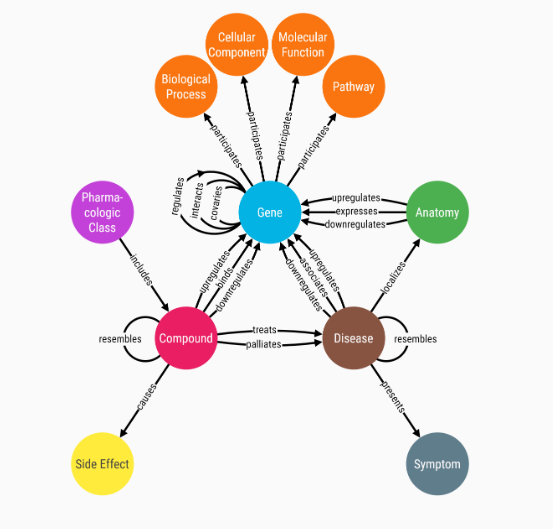
\includegraphics{images/hetionet_schema.PNG}
    \caption{Hetionet graph schema.}
\end{figure}    

\subsubsection{ETL Phases}

The pipeline loads data in two layers, a bronze layer with unfiltered nodes, and a silver layer with nodes filtered by significance according to Himmelstein et al. (eLife 2017). Details on the silver layer are in section \ref{subsubsec:hetionet_silver_layiuer}.

\begin{enumerate}
    \item \textbf{Extract} --- Download source files (nodes TSV, edges SIF.gz, Zenodo DWPC/perm stats)
    \item \textbf{Significance} --- Compute DWPC $p$-values for every edge (gamma-hurdle model, cached to \texttt{pkl})
    \item \textbf{Transform} --- Deduplicate edges, batch by kind/metaedge, stamp \texttt{owner\_id}
    \item \textbf{Connect + Schema} --- Connect to Neo4j via \texttt{NeoHandler}, create indexes and constraints
    \item \textbf{Truncate} --- Delete owner's existing data (bronze + silver)
    \item \textbf{Load Bronze} --- ALL nodes and ALL edges with \texttt{dwpc}/\texttt{p\_value} as relationship properties
    \item \textbf{Silver Layer} --- Create significance-filtered duplicate edges ($p < 0.05$, orphan rescue)
    \item \textbf{Validate} --- Bronze + silver validation, cross-check source file counts vs Neo4j
\end{enumerate}

\subsubsection{Silver layer logic}
\label{subsubsec:hetionet_silver_layer}
Degree-Weighted Path Count (DWPC) p-value filtering — the published gold-standard from Himmelstein et al. (eLife 2017, 700+ citations; GigaScience 2023). The p-value measures edge specificity: "is this connection surprising given the network's degree structure?" We're not removing false edges — we're selecting edges specific enough to test real clinical knowledge.
 
No pre-computed p-value table exists in Hetionet GitHub, Zenodo records, het.io API, JSON or source data. They must be computed using the authors' published data and method:

 \begin{enumerate}
    \item DWPC values — pulled from pre-computed sparse matrices on Zenodo 3978766 (dwpcs_length-1_damping-0.5.zip, 11.7 MB). One matrix per metaedge type containing the observed degree-weighted path count for every node pair.
    \item Null distribution stats — pulled from pre-computed permutation summaries on Zenodo 3978766 (degree-grouped-perms_length-1_damping-0.5.zip, 16.1 MB). Summary statistics (mean, sd, nnz) from 200 XSwap-permuted networks, grouped by source/target degree.
    \item P-values — calculated by us using the gamma-hurdle model:
    \begin{equation}
    p = (\text{nnz}/n) \times \Gamma_{\text{upper}}(\alpha, \beta \times \text{dwpc})
    \end{equation}
    where $\alpha$ and $\beta$ are fit from the permutation stats. This is the exact formula from the hetmatpy package and the published papers.
  \end{enumerate}

 We applied a standard significance cutoff of $p < 0.05$ across all 24 edge types without exception. To maintain network integrity, we implemented an "orphan protection" protocol: any node that lost all its connections during filtering had its single most significant edge (the one with the lowest p-value) restored. 
 Finally, both the DWPC and the associated p-values were stored directly as edge properties within the Neo4j database to ensure full transparency and reproducibility for downstream analysis.


\subsubsection{Node counts}

\begin{table}[H]
\centering
\renewcommand{\arraystretch}{1.2}
\begin{tabular}{|l|l|}
\hline
\textbf{Metric} & \textbf{Count} \\ \hline
Total nodes & 47,031 \\ \hline
Bronze edges & 2,250,197 \\ \hline
Silver edges ($p < 0.05$) & $\sim$882,634 ($\sim$39\%) \\ \hline
Node types & 11 \\ \hline
Edge types & 24 \\ \hline
Largest node type & Gene (20,945) \\ \hline
Largest edge type & GpBP (559,504) \\ \hline
\end{tabular}
\caption{Expected node and edge counts for Hetionet layers.}
\end{table}